\documentclass[border=6pt]{standalone}
\usepackage{tikz}
\usetikzlibrary{arrows.meta,positioning,calc,shapes.misc}
\usepackage[T1]{fontenc}
\usepackage{helvet}
\renewcommand{\familydefault}{\sfdefault}
\definecolor{ink}{HTML}{1F2A37}
\definecolor{blue}{HTML}{2F6DB5}
\definecolor{teal}{HTML}{1F8A70}
\definecolor{amber}{HTML}{C97B14}
\definecolor{grey}{HTML}{8A94A6}
\definecolor{panel}{HTML}{F3F5F8}
\begin{document}
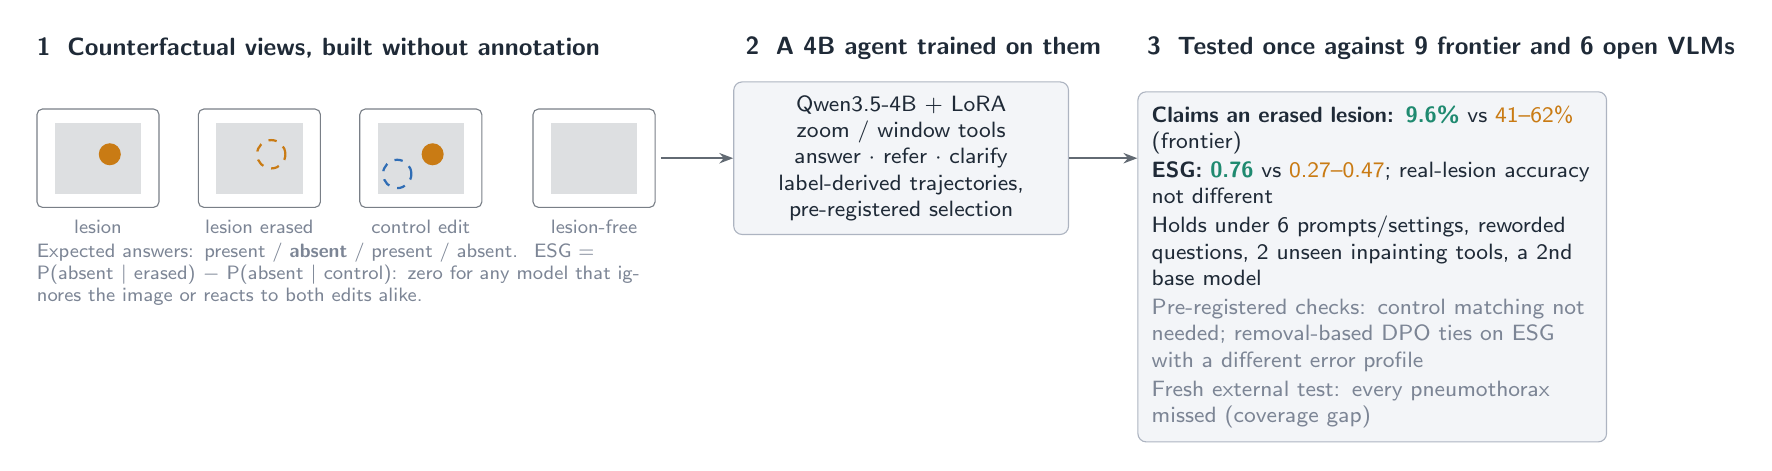
\begin{tikzpicture}[
  font=\footnotesize, text=ink,
  box/.style={draw=grey!70, fill=panel, rounded corners=3pt, inner sep=5pt, align=center, minimum height=1.1cm},
  img/.style={draw=ink!60, fill=white, rounded corners=2pt, minimum width=1.55cm, minimum height=1.25cm, inner sep=2pt, align=center},
  arr/.style={-{Stealth[length=5pt]}, thick, ink!70},
  lab/.style={font=\scriptsize, text=grey!90!black}
]
% ---- 1. counterfactual views ----
\node[font=\small\bfseries, anchor=west] (t1) at (0,3.3) {1\; Counterfactual views, built without annotation};
\node[img] (orig) at (0.9,1.9) {};
\fill[ink!15] (orig.center) ++(-0.55,-0.45) rectangle ++(1.1,0.9);
\fill[amber] (orig.center) ++(0.15,0.05) circle (0.14);
\node[lab, below=1pt of orig] {lesion};
\node[img] (erased) at (2.95,1.9) {};
\fill[ink!15] (erased.center) ++(-0.55,-0.45) rectangle ++(1.1,0.9);
\draw[amber, dashed, thick] (erased.center) ++(0.15,0.05) circle (0.18);
\node[lab, below=1pt of erased] {lesion erased};
\node[img] (ctrl) at (5.0,1.9) {};
\fill[ink!15] (ctrl.center) ++(-0.55,-0.45) rectangle ++(1.1,0.9);
\fill[amber] (ctrl.center) ++(0.15,0.05) circle (0.14);
\draw[blue, dashed, thick] (ctrl.center) ++(-0.3,-0.2) circle (0.18);
\node[lab, below=1pt of ctrl] {control edit};
\node[img] (neg) at (7.2,1.9) {};
\fill[ink!15] (neg.center) ++(-0.55,-0.45) rectangle ++(1.1,0.9);
\node[lab, below=1pt of neg] {lesion-free};
\node[lab, text width=8.0cm, align=left, anchor=north west] at (0,0.95)
  {Expected answers: present / \textbf{absent} / present / absent. \;ESG = P(absent $|$ erased) $-$ P(absent $|$ control): zero for any model that ignores the image or reacts to both edits alike.};

% ---- 2. agent ----
\node[font=\small\bfseries, anchor=west] (t2) at (9.0,3.3) {2\; A 4B agent trained on them};
\node[box, text width=3.9cm] (agent) at (11.1,1.9)
  {Qwen3.5-4B + LoRA\\ zoom / window tools\\ answer $\cdot$ refer $\cdot$ clarify\\ label-derived trajectories, pre-registered selection};
\draw[arr] (8.05,1.9) -- (agent.west);

% ---- 3. results ----
\node[font=\small\bfseries, anchor=west] (t3) at (14.1,3.3) {3\; Tested once against 9 frontier and 6 open VLMs};
\node[box, text width=5.6cm, align=left, anchor=north west] (res) at (14.1,2.75)
  {\textbf{Claims an erased lesion:} \textcolor{teal}{\textbf{9.6\%}} vs \textcolor{amber}{41--62\%} (frontier)\\[1pt]
   \textbf{ESG:} \textcolor{teal}{\textbf{0.76}} vs \textcolor{amber}{0.27--0.47}; real-lesion accuracy not different\\[1pt]
   Holds under 6 prompts/settings, reworded questions, 2 unseen inpainting tools, a 2nd base model\\[1pt]
   \textcolor{grey!90!black}{Pre-registered checks: control matching not needed; removal-based DPO ties on ESG with a different error profile}\\[1pt]
   \textcolor{grey!90!black}{Fresh external test: every pneumothorax missed (coverage gap)}};
\draw[arr] (agent.east) -- (res.west |- agent.east);
\end{tikzpicture}
\end{document}
